\begin{figure}[!ht]
\centering
\resizebox{\columnwidth}{!}{
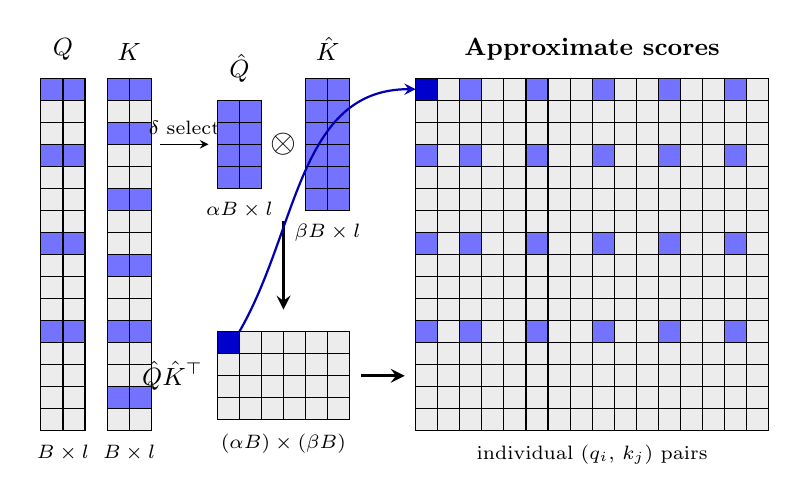
\begin{tikzpicture}
  \def\cell{0.28}
  \colorlet{hilightA}{blue!55}
  \colorlet{hilightFocus}{blue!80!black}
  \colorlet{plain}{gray!15}

  % Q anchors: rows 0, 3, 7, 11   (4 of 16)
  % K anchors: rows 0, 2, 5, 8, 11, 14  (6 of 16)

  %--- Full Q (16 rows × 2 cols) ---
  \foreach \r in {0,...,15} {
    \pgfmathtruncatemacro{\isanchor}{
      (((\r==0)+(\r==3)+(\r==7)+(\r==11))>0) ? 1 : 0
    }
    \foreach \c in {0,1} {
      \ifnum\isanchor=1 \fill[hilightA] \else \fill[plain] \fi
        ({\c*\cell},{-\r*\cell}) rectangle ({(\c+1)*\cell},{(-\r-1)*\cell});
      \draw ({\c*\cell},{-\r*\cell}) rectangle ({(\c+1)*\cell},{(-\r-1)*\cell});
    }
  }
  \node[above, font=\small\bfseries] at ({1*\cell}, 0.1)             {$Q$};
  \node[below, font=\scriptsize]     at ({1*\cell},{-16*\cell-0.05}) {$B \times l$};

  %--- Full K (16 rows × 2 cols) ---
  \foreach \r in {0,...,15} {
    \pgfmathtruncatemacro{\isanchor}{
      (((\r==0)+(\r==2)+(\r==5)+(\r==8)+(\r==11)+(\r==14))>0) ? 1 : 0
    }
    \foreach \c in {0,1} {
      \ifnum\isanchor=1 \fill[hilightA] \else \fill[plain] \fi
        ({(3+\c)*\cell},{-\r*\cell}) rectangle ({(4+\c)*\cell},{(-\r-1)*\cell});
      \draw ({(3+\c)*\cell},{-\r*\cell}) rectangle ({(4+\c)*\cell},{(-\r-1)*\cell});
    }
  }
  \node[above, font=\small\bfseries] at ({4*\cell}, 0.1)             {$K$};
  \node[below, font=\scriptsize]     at ({4*\cell},{-16*\cell-0.05}) {$B \times l$};

  %--- Delta-select arrow ---
  \draw[-{stealth}] ({5.4*\cell},{-3*\cell}) -- ({7.6*\cell},{-3*\cell});
  \node[above, font=\scriptsize] at ({6.5*\cell},{-3*\cell}) {$\delta$ select};

  %--- \hat{Q} (4 rows × 2 cols) ---
  \foreach \r in {0,...,3} {
    \foreach \c in {0,1} {
      \fill[hilightA]
        ({(8+\c)*\cell},{-(1+\r)*\cell}) rectangle ({(9+\c)*\cell},{-(2+\r)*\cell});
      \draw ({(8+\c)*\cell},{-(1+\r)*\cell}) rectangle ({(9+\c)*\cell},{-(2+\r)*\cell});
    }
  }
  \node[above, font=\small\bfseries] at ({9*\cell},{-1*\cell+0.1})       {$\hat{Q}$};
  \node[below, font=\scriptsize]     at ({9*\cell},{-5*\cell-0.05}) {$\alpha B \times l$};

  %--- ⊗ ---
  \node[font=\large] at ({11*\cell},{-3*\cell}) {$\otimes$};

  %--- \hat{K} (6 rows × 2 cols) ---
  \foreach \r in {0,...,5} {
    \foreach \c in {0,1} {
      \fill[hilightA]
        ({(12+\c)*\cell},{-\r*\cell}) rectangle ({(13+\c)*\cell},{-(1+\r)*\cell});
      \draw ({(12+\c)*\cell},{-\r*\cell}) rectangle ({(13+\c)*\cell},{-(1+\r)*\cell});
    }
  }
  \node[above, font=\small\bfseries] at ({13*\cell}, 0.1)       {$\hat{K}$};
  \node[below, font=\scriptsize]     at ({13*\cell},{-6*\cell-0.05}) {$\beta B \times l$};

  %--- Downward Flow Arrow ---
  \draw[-{stealth}, very thick] ({11*\cell},{-6.5*\cell}) -- ({11*\cell},{-10.5*\cell});

  %--- (αB)×(βB) result matrix: 4 rows × 6 cols ---
  \foreach \r in {0,...,3} {
    \foreach \c in {0,...,5} {
      \pgfmathtruncatemacro{\isFocus}{(\r==0)*(\c==0)}
      \ifnum\isFocus=1
        \fill[hilightFocus]
      \else
        \fill[plain]
      \fi
        ({(8+\c)*\cell},{-(11.5+\r)*\cell}) rectangle ({(9+\c)*\cell},{-(12.5+\r)*\cell});
      \draw ({(8+\c)*\cell},{-(11.5+\r)*\cell}) rectangle ({(9+\c)*\cell},{-(12.5+\r)*\cell});
    }
  }
  \node[left, font=\small\bfseries]  at ({7.8*\cell},{-13.5*\cell})    {$\hat{Q}\hat{K}^\top$};
  \node[below, font=\scriptsize]     at ({11*\cell},{-15.5*\cell-0.05}) {$(\alpha B)\times(\beta B)$};

  %--- Rightward Flow Arrow ---
  \draw[-{stealth}, very thick] ({14.5*\cell},{-13.5*\cell}) -- ({16.5*\cell},{-13.5*\cell});

  %--- 16×16 full score matrix ---
  \foreach \r in {0,...,15} {
    \foreach \c in {0,...,15} {
      \pgfmathtruncatemacro{\isHL}{
        (((\r==0)+(\r==3)+(\r==7)+(\r==11))>0) *
        (((\c==0)+(\c==2)+(\c==5)+(\c==8)+(\c==11)+(\c==14))>0)
      }
      \pgfmathtruncatemacro{\isFocus}{(\r==0)*(\c==0)}
      \ifnum\isFocus=1
        \fill[hilightFocus]
      \else
        \ifnum\isHL=1
          \fill[hilightA]
        \else
          \fill[plain]
        \fi
      \fi
        ({(17+\c)*\cell},{-\r*\cell}) rectangle ({(18+\c)*\cell},{-(1+\r)*\cell});
      \draw ({(17+\c)*\cell},{-\r*\cell}) rectangle ({(18+\c)*\cell},{-(1+\r)*\cell});
    }
  }
  \node[above, font=\small\bfseries] at ({25*\cell}, 0.1) {Approximate scores};
  \node[below, font=\scriptsize]     at ({25*\cell}, {-16*\cell-0.05}) {individual $(q_i,\,k_j)$ pairs};

  %--- Arrow from result cell (0,0) to B×B position (0,0) ---
  \draw[-{stealth}, thick, blue!70!black]
      ({9*\cell},{-11.5*\cell})
      to[out=60, in=180]
      ({17*\cell},{-0.5*\cell});

\end{tikzpicture}
}
\caption{Delta-based tile scoring. Delta pre-processing selects content-adaptive anchors (blue) from $Q$ and $K$ independently, producing $\hat{Q}$ and $\hat{K}$. Their product gives an $(\alpha B)\times(\beta B)$ score matrix; each entry (highlighted cell, arrow) corresponds to a single dot product at one position in the full $B\times B$ score tile.}
\label{fig:delta_tile_scoring}
\end{figure}
